% Intended LaTeX compiler: pdflatex
\documentclass[10pt,a4paper,UTF8]{article}
\usepackage{zclorg}
\date{}
\title{正交补与极小化问题}
\hypersetup{
 pdfauthor={},
 pdftitle={正交补与极小化问题},
 pdfkeywords={},
 pdfsubject={},
 pdfcreator={Emacs 25.0.50.1 (Org mode 9.0.6)},
 pdflang={English}}
\begin{document}

\maketitle
\tableofcontents
\titlepic{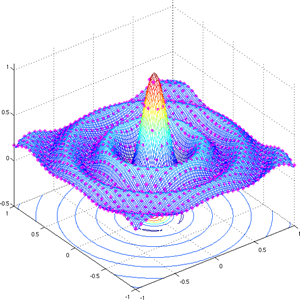
\includegraphics[scale=0.25]{../../img/sinc.PNG}}

\section{正交补}
\label{sec:org0110aba}


\begin{definition}
设\(U\)是\(V\)的子集,则\(U\)的正交补(记为\(U^{\perp}\))是由\(V\)中与\(U\)的每个向量都正交的那些向量组成的集合:
\begin{equation}
\label{eq:1}
U^{\perp} = \{v\in V: \forall~u\in U, \langle v,u \rangle = 0  \}
\end{equation}
\end{definition}

若\(U\)是\(\mathbf{R}^{3}\)中的直线,则\(U^{\perp}\)是垂直于\(U\)且包含原点的平面。若\(U\)是\(\mathbf{R}^{3}\)中的平面,则\(U^{\perp}\)是垂直于\(U\)且包含原点的直线。

\begin{theorem}
\begin{enumerate}
\item 若\(U\)是\(V\)的子集,则\(U^{\perp}\)是\(V\)的子空间。
\item \(\{0\}^{\perp} = V\)
\item \(V^{\perp} = \{0\}\)
\item 若\(U\)是\(V\)的子集,则\(U\cap U^{\perp} = \{0\}\)
\item 若\(U\)和\(W\)均为\(V\)的子集且\(U\subset W\),则\(W^{\perp} \subset U^{\perp}\)
\end{enumerate}
\end{theorem}

\begin{proof}
\begin{enumerate}
\item 设\(U\)是\(V\)的子集,则对每个\(u\in U\)均有\(\langle 0,u \rangle = 0\),于是\(0 \in U^{\perp}\). 设\(v,w\in U^{\perp}\),若\(u\in U\),则:\[ \langle v+w,u \rangle = \langle v,u \rangle  + \langle w,u \rangle  = 0\] 因此\(v+w\in U^{\perp}\),所以在加法下\(U^{\perp}\)是封闭的。
\end{enumerate}

类似的对于\(v\in U^{\perp}\),有\(\langle \lambda v,u \rangle = \lambda \langle v,u \rangle  = 0\)这说明\(U^{\perp}\)在标量乘法下是封闭的。

所以\(U^{\perp}\)是\(V\)的子空间。

\begin{enumerate}
\item \(\forall v\in V\), 均有:\(\langle v,0 \rangle = 0\) ,所以\(\{0\}^{\perp} = V\)
\item 假设\(v\in V^{\perp}\),则\(\langle v,v \rangle  = 0\),则\(v=0\),所以\(V^{\perp} = 0\)
\item 假设\(v\in U\cap U^{\perp}\),则有\(\langle v,v \rangle   = 0\),则\(v = 0\),所以\(U \cap U^{\perp} = \{0\}\)
\item 设\(U,W\)均为\(V\)的子集,则对于\(v\in W^{\perp}\),说明对于\(\forall~u\in W\),都有\(\langle v,u \rangle = 0\),这表明对于每个\(u\in U\),都有\(\langle v,u \rangle  = 0\),所以\(v \in U^{\perp}\),所以有\(W^{\perp} \subset U^{\perp}\)
\end{enumerate}
\end{proof}

若\(U,W\)均为\(V\)的子空间,并且\(V\)中的每个元素都可以唯一的写成\(U\)中的一个向量与\(W\)中的一个向量的和,则\(V\)是\(U\)和\(W\)的直和,记为\(V = U\oplus W\)

\begin{theorem}
设\(U\)是\(V\)的有限维子空间,则\(V = U \oplus U^{\perp}\)
\end{theorem}

\begin{proof}
首先证明:
\[V = U + U^{\perp}\]
假设\(v\in V\),并设\(e_{1},\ldots ,e_{m}\)是\(U\)的规范正交基,则:
\begin{equation}
\label{eq:2}
v = \underbrace{\langle v,e_{1} \rangle e_{1} + \ldots  + \langle v,e_{m} \rangle e_{m}}_{u} +\underbrace{ v -\langle v,e_{1} \rangle e_{1} - \ldots  - \langle v,e_{m} \rangle e_{m}}_{w}
\end{equation}
显然\(u\in U\),因为\(e_{1},\ldots ,e_{m}\)是\(U\)的一个规范正交基,所以对每个\(j=1,\ldots ,m\)均有:
\begin{equation}
\label{eq:3}
\langle w,e_{j} \rangle  = \langle v,e_{j} \rangle  - \langle v,e_{j} \rangle = 0
\end{equation}

所以\(w\)正交于\(\mathrm{span}(e_{1},\ldots ,e_{m})\)中的每个向量。也就是说\(w\in U^{\perp}\),于是\(v = u + w\)其中\(u\in U,w\in U^{\perp}\)
另外因为\(U\cap U^{\perp} = \{0\}\),所以\[V= U \oplus U^{\perp}\]
\end{proof}
\begin{theorem}
设\(V\)是有限维的且\(U\)是\(V\)的子空间,则\(\dim U^{\perp} = \dim V - \dim U\)
\end{theorem}

\begin{theorem}
\(U\)是\(V\)的有限维子空间,则\(U= (U^{\perp})^{\perp}\)
\end{theorem}

\begin{proof}
首先证明\(U\subset (U^{\perp})^{\perp}\)。设\(u\in U\),则对每个\(v\in U^{\perp}\),均有\(\langle v,u \rangle  = 0\).因为 \(u\)正交与\(U^{\perp}\)中的向量,所以\(u\in (U^{\perp})^{\perp}\)

然后我证明另一个方向。设\(v\in (U^{\perp})^{\perp}\)。设\(v\in (U^{\perp})^{\perp}\)令\(v=u+w\),其中\(u\in U\),且\(w\in U^{\perp}\),从而\(v-u = w\in U^{\perp}\)。因为\(v\in (U^{\perp})^{\perp}\)且\(u\in (U^{\perp})^{\perp}\),所以\(v-u\in (U^{\perp})^{\perp}\),所以\(v-u\in U^{\perp} \cap  (U^{\perp})^{\perp}\)。这表明\(v-u\)与自身正交。从而\(v-u=0\),即\(v=u\),于是\(v\in U\),因此\((U^{\perp})^{\perp} \subset U\)
\end{proof}

\begin{definition}
设\(U\)是\(V\)的有限维子空间。定义\(V\)到\(U\)上的正交投影为如下算子\(P_{U} \in \mathcal{L}(V)\):对\(v\in V\),将其写成\(v= u+w\),其中\(u\in U,w\in U^{\perp}\),则\(P_{U}v = u\)
\end{definition}

直和分解\(V =  U \oplus U^{\perp}\)表明每个\(v\in V\)可唯一的写成\(v = u + w\),其中\(u\in U\)且\(w\in U^{\perp}\),于是\(P_{U}v\)定义合理。

\begin{instance}
设\(x\in V\),\(x\neq 0\)且\(U = \mathrm{span}(x)\),证明对每个\(x\in V\)均有:
\begin{equation}
\label{eq:4}
P_{U}v = \frac{ \langle v,x \rangle  }{ \| x \|^{2} } x
\end{equation}
已知\(\forall~v\in V\)都可以写为:
\begin{equation}
\label{eq:5}
v= \frac{ \langle v,x \rangle  }{ \| x \|^{2} } x  + (v - \frac{ \langle v,x \rangle  }{ \| x \|^{2} } x)
\end{equation}
上式第一项和第二项是互相垂直的。第一项属于\(\mathrm{span}(x)\),第二项正交与\(x\),从而第二项属于\(U^{\perp}\)。所以\(P_{U}v\)等于上式右端第一项。
\end{instance}
接下来给出几条正交投影\(P_{U}\)的性质:
设\(U\)是\(V\)的有限维子空间且\(v\in V\),则:
\begin{enumerate}
\item \(P_{U}\in \mathcal{L}(V)\)
\item \(\forall ~u, P_{U}u = u\)
\item \(\forall ~w\in U^{\perp},P_{U}w = 0\)
\item \(\mathrm{range} P_{U} = U\)
\item \(\mathrm{null}P_{U} = U^{\perp}\)
\item \(v-P_{U}v \in U^{\perp}\)
\item \((P_{U})^{2} = P_{U}\)
\item \(\| (P_{U})v  \|  \leq \| v \|\)
\item 对\(U\)的每个规范正交基\(e_{1},\ldots ,e_{n}\)均有\(P_{U}v = \langle v,e_{1} \rangle e_{1} + \ldots + \langle v,e_{m} \rangle e_{m}\)
\end{enumerate}

\begin{proof}
为了证明\(P_{U}\)是\(V\)上的线性映射,设\(v_{1},v_{2}\in V\),设:
\begin{equation}
\label{eq:6}
v_{1} = u_{1} + w_{1}, v_{2} = u_{2} + w_{2}
\end{equation}
其中\(u_{1},u_{2}\in U\),\(w_{1},w_{2}\in U^{\perp}\),则\(P_{U}v_{1} = u_{1},P_{U}v_{2} = u_{2}\),从而:
\[v_{1} + v_{2} = u_{1} + u_{2} + w_{1} + w_{2}\]
其中\(u_{1} + u_{2}\in U\),且\(w_{1} + w_{2}\in U^{\perp}\),所以\(P_{U}(v_{1}+ v_{2}) = u_{1} + u_{2} = P_{U}v_{1} + P_{U}v_{2}\)
类似的有,设\(\lambda\in \mathbf{F}\),若\(v= u + w\),其中\(u\in U\)且\(w\in U^{\perp}\),则\(\lambda v = \lambda u + \lambda w\),其中\(\lambda u\in U, \lambda w\in U^{\perp}\),于是\(P_{U}(\lambda v) = \lambda u = \lambda P_{U}v\),因此\(P_{U}\)是\(V\)到\(V\)的线性映射。
\end{proof}
\begin{proof}
设\(u\in U\),则\(u = u + 0\),则其中\(u\in U,0\in U^{\perp}\),所以\(P_{U}u = u\)
\end{proof}
\begin{proof}
设\(w\in U^{\perp}\),则\(w = 0 + w\),则其中\(0\in U,w\in U^{\perp}\),所以\(P_{U}w = 0\)
\end{proof}
\begin{proof}
由\(P_{U}\)的定义可知\(\mathrm{range}(P_{U})\subset U\)。由上面第二步可知\(U\subset \mathrm{range}P_{U}\),于是\(\mathrm{range}P_{U} = U\)
\end{proof}

\begin{proof}
因为\(U^{\perp}\subset \mathrm{null}P_{U}\)。另外,\(\forall~v\in \mathrm{null}P_{u}\)则\(v= 0+ v\),其中\(0\in U,v\in U^{\perp}\),因此\(\mathrm{null}P_{U}\subset U^{\perp}\)
\end{proof}

\begin{proof}
若\(v = u + w\),其中\(u\in U\),且\(w\in U^{\perp}\),则:
\[v- P_{U}v= v-u = w\in U^{\perp} \]
\end{proof}

\begin{proof}
若\(v = u+w\),其中\(u\in U\),且\(w\in U^{\perp}\),则:
\begin{equation}
\label{eq:7}
(P_{U})^{2}v = P_{U}(P_{U}v) = P_{U}u= u= P_{U}v
\end{equation}
所以\(P_{U}^{2} = P_{U}\)
\end{proof}

\begin{proof}
若\(v = u+w\),其中\(u\in U\),且\(w\in U^{\perp}\),则:
\[ \| P_{U}v \|^{2} = \| u \|^{2} \leq \| u \|^{2} + \| w \|^{2} = \| v \|^{2}  \]
\end{proof}
\section{极小化问题}
\label{sec:org24c64c4}


经常会遇到这样的问题:给定\(V\)的子空间\(U\)和点\(v\in V\),求点\(u\in U\)使得\(\| v-u \|\)最小。通过正交投影可以完美解决这个问题。

\begin{theorem}
设\(U\)是\(V\)的最小子空间,\(v\in V\),且\(u\in U\),则:
\begin{equation}
\label{eq:8}
\| v - P_{U}v \| \leq \| v - u \|
\end{equation}
当且仅当\(P_{U}v = u\)时等号成立。
\end{theorem}

\begin{proof}
我们有:
\begin{eqnarray}
\label{eq:9}
\| v- P_{U}v \|^{2} &\leq&    \| v- P_{U}v \|^{2} + \|  P_{U}v - u \|^{2}
&=&  \| v - P_{U}v + P_{U}v - u \|^{2} \\
&=& \| v - u \|^{2}
\end{eqnarray}
上式的第一个不等号成立是因为\(\| P_{U}v - u \|^{2}\)是一个非负实数,第二个等号成立是因为勾股定理,第三个等式成立是简单的消元计算。把上式两端开平方即可。
\end{proof}

上式的证明表明\(P_{U}v\)是\(U\)中离\(v\)最近的点。之前我们又有\(P_{U}v = \langle v,e_{1} \rangle e_{1} + \ldots + \langle v,e_{m} \rangle\),其中\(e_{1},\ldots ,e_{m}\)是\(U\)的规范正交基。
\end{document}